\documentclass{beamer}

\usepackage{algorithm}
\usepackage{algpseudocode}
\usepackage{mathtools}

\usefonttheme{serif}
\usepackage{dsfont}
\setbeamersize{text margin left=5pt, text margin right=5pt}

\newcommand{\bgk}[1]{\boldsymbol{#1}}

\newcommand{\bzero}{\bgk{0}}
\newcommand{\bone}{\bgk{1}}

\newcommand{\balpha}{\bgk{\alpha}}
\newcommand{\bnu}{\bgk{\nu}}
\newcommand{\bbeta}{\bgk{\beta}}
\newcommand{\bxi}{\bgk{\xi}}
\newcommand{\bgamma}{\bgk{\gamma}} 
\newcommand{\bo}{\bgk{o }}
\newcommand{\bdelta}{\bgk{\delta}}
\newcommand{\bpi}{\bgk{\pi}}
\newcommand{\bepsilon}{\bgk{\epsilon}} 
\newcommand{\bvarepsilon}{\bgk{\varepsilon}} 
\newcommand{\brho}{\bgk{\rho}}
\newcommand{\bvarrho}{\bgk{\varrho}}
\newcommand{\bzeta}{\bgk{\zeta}}
\newcommand{\bsigma}{\bgk{\sigma}}
\newcommand{\boldeta}{\bgk{\eta}}
\newcommand{\btay}{\bgk{\tau}}
\newcommand{\btheta}{\bgk{\theta}}
\newcommand{\bvertheta}{\bgk{\vartheta}}
\newcommand{\bupsilon}{\bgk{\upsilon}}
\newcommand{\biota}{\bgk{\iota}}
\newcommand{\bphi}{\bgk{\phi}}
\newcommand{\bvarphi}{\bgk{\varphi}}
\newcommand{\bkappa}{\bgk{\kappa}}
\newcommand{\bchi}{\bgk{\chi}}
\newcommand{\blambda}{\bgk{\lambda}}
\newcommand{\bpsi}{\bgk{\psi}}
\newcommand{\bmu}{\bgk{\mu}}
\newcommand{\bomega}{\bgk{\omega}}

\newcommand{\bA}{\bgk{A}}
\newcommand{\bDelta}{\bgk{\Delta}}
\newcommand{\bLambda}{\bgk{\Lambda}}
\newcommand{\bSigma}{\bgk{\Sigma}}
\newcommand{\bOmega}{\bgk{\Omega}}
\newcommand{\bPsi}{\bgk{\Psi}}

\newcommand{\bvec}[1]{\mathbf{#1}}

\newcommand{\va}{\bvec{a}}
\newcommand{\vb}{\bvec{b}}
\newcommand{\vc}{\bvec{c}}
\newcommand{\vd}{\bvec{d}}
\newcommand{\ve}{\bvec{e}}
\newcommand{\vf}{\bvec{f}}
\newcommand{\vg}{\bvec{g}}
\newcommand{\vh}{\bvec{h}}
\newcommand{\vi}{\bvec{i}}
\newcommand{\vj}{\bvec{j}}
\newcommand{\vk}{\bvec{k}}
\newcommand{\vl}{\bvec{l}}
\newcommand{\vm}{\bvec{m}}
\newcommand{\vn}{\bvec{n}}
\newcommand{\vo}{\bvec{o}}
\newcommand{\vp}{\bvec{p}}
\newcommand{\vq}{\bvec{q}}
\newcommand{\vr}{\bvec{r}}
\newcommand{\vs}{\bvec{s}}
\newcommand{\vt}{\bvec{t}}
\newcommand{\vu}{\bvec{u}}
\newcommand{\vv}{\bvec{v}}
\newcommand{\vw}{\bvec{w}}
\newcommand{\vx}{\bvec{x}}
\newcommand{\vy}{\bvec{y}}
\newcommand{\vz}{\bvec{z}}

\newcommand{\vA}{\bvec{A}}
\newcommand{\vB}{\bvec{B}}
\newcommand{\vC}{\bvec{C}}
\newcommand{\vD}{\bvec{D}}
\newcommand{\vE}{\bvec{E}}
\newcommand{\vF}{\bvec{F}}
\newcommand{\vG}{\bvec{G}}
\newcommand{\vH}{\bvec{H}}
\newcommand{\vI}{\bvec{I}}
\newcommand{\vJ}{\bvec{J}}
\newcommand{\vK}{\bvec{K}}
\newcommand{\vL}{\bvec{L}}
\newcommand{\vM}{\bvec{M}}
\newcommand{\vN}{\bvec{N}}
\newcommand{\vO}{\bvec{O}}
\newcommand{\vP}{\bvec{P}}
\newcommand{\vQ}{\bvec{Q}}
\newcommand{\vR}{\bvec{R}}
\newcommand{\vS}{\bvec{S}}
\newcommand{\vT}{\bvec{T}}
\newcommand{\vU}{\bvec{U}}
\newcommand{\vV}{\bvec{V}}
\newcommand{\vW}{\bvec{W}}
\newcommand{\vX}{\bvec{X}}
\newcommand{\vY}{\bvec{Y}}
\newcommand{\vZ}{\bvec{Z}}

\usepackage{subcaption}
\newcommand{\bitem}{\item[$\bullet$]}

\usepackage{xcolor}
\usepackage[utf8]{inputenc}
\DeclareFontEncoding{LS1}{}{}
\DeclareFontSubstitution{LS1}{stix}{m}{n}
\DeclareSymbolFont{symbols2}{LS1}{stixfrak} {m} {n}
\DeclareMathSymbol{\operp}{\mathbin}{symbols2}{"A8}
\setbeamertemplate{navigation symbols}{}

\usepackage{lipsum}

\newtheorem{proposition}[theorem]{Proposition}

\newcommand\blfootnote[1]{%
  \begingroup
  \renewcommand\thefootnote{}\footnote{#1}%
  \addtocounter{footnote}{-1}%
  \endgroup
}

\addtobeamertemplate{navigation symbols}{}{%
    \usebeamerfont{footline}%
    \usebeamercolor[fg]{footline}%
    \hspace{1em}%
    \insertframenumber/\inserttotalframenumber
}

\title{
Sketching Krylov Subspace Methods\\ -- Linear Systems -- \\
Lecture 23
}
%\subtitle{Mathematical framework, existence and exactness}

\author{F. M. Faulstich}
\date{04/19/2024}

\begin{document}

\frame{\titlepage}


\begin{frame}{Conjugate Gradient}

\begin{itemize}
    \bitem Method of steepest descent\\
    \pause
    $\Rightarrow$ Rewrite the problem as minimization:
    $$
    \min_{\vx \in \mathbb{R}^n} \frac{1}{2}\vx^\top \vA \vx - \vx^\top \vb
    $$
    for $\vA \in \mathbb{H}_n$ and $\vA \succ \bzero$.\\
    \pause
    $\Rightarrow$ ``walk'' in the direction of the steepest descent\\
    $\Rightarrow$ Very intuitive but -- in general -- not optimal
    \pause
    \bitem Different idea:\\
    \pause
    $\vA$-conjugate the gradient w.r.t.~the previous search directions\\
    $\Rightarrow$ conjugate gradient (CG) method
    \pause
    \bitem CG is a Krylov subspace method, i.e., $\vx_k \in \mathcal{K}_k$
    \bitem The search direction at k$th$ iteration is optimal
    $$
    \Vert \vx_* - \vx_k \Vert_{\vA} = \min_{\vx \in \mathcal{K}_k} \Vert \vx_* - \vx \Vert_{\vA}
    $$
    and $\Vert \vx_* - \vx_\ell\Vert_{\vA} = 0 $ for some $\ell \leq n$
\end{itemize}
    
\end{frame}

\begin{frame}{Generalized Minimal Residual Method}

\only<1>{
\begin{center}
Question: What if $\vA\in\mathbb{R}^{n\times n}$ is a general matrix?
\end{center}
}

\only<2>{
\begin{itemize}
    \bitem Following the idea of Krylov subspace methods we seek 
    $$
    \min_{\vx \in \vx_0 + \mathcal{K}_k({\vA,\vr_0})} \Vert \vb - \vA \vx \Vert
    $$
    where $\mathcal{K}_k({\vA,\vr_0}) = {\rm span}(\vr_0, \vA \vr_0,...,\vA^{k-1} \vr_0)$\\
    (Note that if $\vx_0 = \bzero$, we have $\vr_0 = \vb$)
    \bitem Assume we have an orthonormal basis $\{\vv_1,...,\vv_k\}$ of  $\mathcal{K}_k({\vA,\vr_0})$. Then
    $$
    \vx = \vx_0 + \vV_k \vy
    $$
    for some $\vy \in \mathbb{R}^k$, with $\vV_k = [\vv_1|...|\vv_k] \in\mathbb{R}^{n \times k}$ and 
    $$
    \Vert \vb - \vA \vx \Vert
    =
    \Vert \vb - \vA (\vx_0 + \vV_k \vy) \Vert
    =
    \Vert \vr_0 - \vA \vV_k \vy \Vert
    $$
    hence
    $$
    \min_{\vx \in \vx_0 + \mathcal{K}_k({\vA,\vr_0})} \Vert \vb - \vA \vx \Vert
    =
    \min_{\vy \in \mathbb{R}^k} \Vert \vr_0 - \vA \vV_k \vy \Vert
    $$
    $\Rightarrow$ Ordinary least-squares problem!
\end{itemize}
}
\only<3>{
\begin{itemize}
    \bitem NOTE: This method needs an orthonormal basis of $\mathcal{K}_k({\vA,\vr_0})$\\
    $\Rightarrow$ Vulnerable to an imperfect basis caused by computational errors
\end{itemize}
\begin{center}
Different approaches to computing this basis lead to different ``flavors'' of GMRES
\end{center}
}

\end{frame}


\begin{frame}{GMRES with Arnoldi (Gram-Schmidt)}

\only<1>{
\begin{itemize}
\bitem Arnoldi process:\\
    $\vr_0~\leftarrow$ Initial residual\\
    $\vv_1 = \vr_0 / \Vert \vr_0 \Vert$\\
    $\vV_{1} = [\vv_1]$\\
    For $p=2$ to $k$:\\
    $\qquad \vw_p = (\vI - \vV_{p-1} \vV_{p-1}^\top) \vA \vv_{p-1}$\\
    $\qquad \vv_p = \vw_p / \Vert \vw_p \Vert$\\
    $\qquad \vV_p = [\vV_{p-1}|\vv_p]$
\end{itemize}
}

\only<2>{
\begin{itemize}
    \bitem This yields
    $$
    \vA \vV_k = \vV_{k+1} \vH_k
    $$
    with 
    $$
     \vH_k=
    \begin{bmatrix}
    h_{1,1} & h_{1,2} & \cdots & h_{1,k}\\
    h_{2,1} & h_{2,2} & \cdots & h_{2,k}\\
    0 & h_{3,2} & h_{3,3} & \vdots\\
    \vdots & \ddots & \ddots & \\
    0 & & h_{k,k-1} & h_{k,k}\\
    0 & & 0 & h_{k+1,k}
    \end{bmatrix}
    $$
\end{itemize}
}

\only<3>{
\begin{itemize}
    \bitem Note that
    $$
    \vr_0 = \Vert \vr_0 \Vert \vv_1 =: \beta \vv_1
    $$
    \bitem Hence
    $$
    \Vert \vr_0 - \vA \vV_k \vy \Vert
    =
    \Vert \vr_0 - \vV_{k+1} \vH_k \vy \Vert
    =
    \Vert \vV_{k+1}(\beta\ve_1 -\vH_k \vy) \Vert
    =
    \Vert \beta\ve_1 -\vH_k \vy \Vert
    $$
    \bitem Thus we seek to solve
    $$
    \min_{\vy \in \mathbb{R}^{k}} \Vert \beta\ve_1 -\vH_k \vy \Vert
    $$
    Using QR factorization of $\vH_k = \vQ_k \vR_k$ we get
    $$
    \min_{\vy \in \mathbb{R}^{k}} \Vert \vQ_k (\beta\vQ_k^\top \ve_1 -\vR_k \vy) \Vert
    =
    \min_{\vy \in \mathbb{R}^{k}} \Vert  \vg_k -\vR_k \vy \Vert
    $$
    The minimum is obtained at $[\vR_k \vy]_{i=1}^{k} = [\vg_k]_{i=1}^{k}$. Hence
    $$
    \min_{\vy \in \mathbb{R}^{k}} \Vert  \vg_k -\vR_k \vy \Vert
    =
    [\vg_k]_{k+1}
    $$
\end{itemize}
}

\end{frame}


\begin{frame}{Make GMRES more stable}

\begin{itemize}
    \bitem Gram-Schmidt may suffer from numerical instabilities!
    \bitem Alternatives exist:
    \begin{itemize}
        \item[] modified Gram Schmidt
        \item[] double Gram-Schmidt
        \item[] Given's rotations
        \item[] Householder
    \end{itemize}
\end{itemize}
    
\end{frame}

\begin{frame}{Computational comparison}


\begin{itemize}
    \bitem N. I. Dravins, Numerical Implementations of the GMRES (2015):
\end{itemize}

\begin{figure}
    \centering
    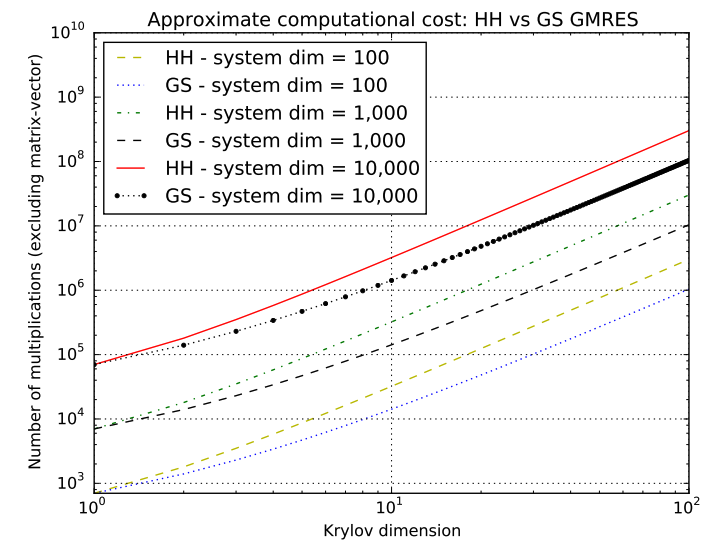
\includegraphics[width = .5\textwidth]{Graphics/HHvsGS_GMRES.png}
\end{figure}
\end{frame}

\begin{frame}{GMRES with Lanczos recurrence}

\begin{itemize}
    \bitem We assume $\vA \in\mathbb{H}_n$
    \bitem Arnoldi process simplifies dramatically:\\
    In every iteration
    $$
    \vw_p = (\vI  - \vv_{p-1}\vv_{p-1}^\top - \vv_{p-2}\vv_{p-2}^\top) \vA \vv_{p-1}
    $$
    \bitem The Lanczos basis yields
    $$
    \vV_k^\top \vA \vV_k = \vJ_k 
    $$
    where $\vJ_k$ is tri-diagonal
\end{itemize}
    
\end{frame}

\begin{frame}{GMRES with Chebyshev recurrence}

\begin{itemize}
    \bitem Sometimes orthogonalization is infeasible all together
    \bitem Assume $\Lambda(\vA) \in [c\pm \delta_x, \pm \delta_y]$, and $\rho := \max \{ \delta_x, \delta_y\}$
    \bitem Chebyshev recurrence:\\
    $\vv_1 = \vr_0/\Vert \vr_0\Vert$\\
    $\vv_2 = (2\rho)^{-1} (\vA -c\vI) \vv_1$\\
    for $p = 3$ to $k$:\\
    $\quad$ $\vv_p = \frac{1}{\rho} \left( (\vA - c\vI)\vv_{p-1} - \frac{\delta_x^2 - \delta_y^2}{4\rho}\vv_{p-2} \right)$\\
    $\quad$ $\vv_{p-2} = \vv_{p-2}/\Vert \vv_{p-2} \Vert$\\
    $\vv_{k-1} = \vv_{k-1}/\Vert \vv_{k-1} \Vert$\\
    $\vv_{k} = \vv_{k}/\Vert \vv_{k} \Vert$
    \bitem Good idea when dealing with large, sparse linear systems, where the coefficient matrix may be ill-conditioned
    \bitem Requires some estimate of the spectrum
\end{itemize}
    
\end{frame}


\begin{frame}{GMRES with sketching}

\begin{itemize}
    \bitem Remember, we basically want to solve
    $$
    \min_{\vy \in \mathbb{R}^k} \Vert \vr_0 - \vA \vV_k \vy\Vert 
    $$
    at every iteration
    % \bitem This is equivalent to:\\
    % Find $\vy$ s.t. 
    % $$
    % (\vA \vV_k)^\top (\vA \vV_k \vy - \vr_0) = 0
    % $$
    \bitem As a least-squares problem it is a natural candidate for sketching
    $$
    \min_{\vy \in \mathbb{R}^k} \Vert \vS(\vr_0 - \vA \vV_k \vy)\Vert 
    $$
    where $\vS \in\mathbb{R}^{d\times n}$ is the sketching matrix
    \begin{itemize}
        \bitem Gaussian
        \bitem SRTT
        \bitem SSE\\
        ~~\vdots
    \end{itemize}
\end{itemize}
    
\end{frame}


\begin{frame}{Comparison sGMRES vs GMRES\footnote{Nakatsukasa and Tropp, arXiv:2111.00113}}
\begin{footnotesize}
\begin{itemize}
    \bitem Comparison of performance of MATLAB GMRES (with and without restarting) against the sGMRES algorithm (with 2-partial
orthogonalization or the Chebyshev basis)
\bitem Sparse linear system $\vA\vx = \vf$, $\vA$ is 2D Laplacian with $n = 10^6$.
\bitem Left: Relative residual and condition number $\kappa_2(AB)$ of the
reduced matrix associated with the $k$-truncated Arnoldi basis. 
\bitem Right: Total runtime including basis
generation. 
\end{itemize}
\end{footnotesize}

\begin{figure}
    \centering
    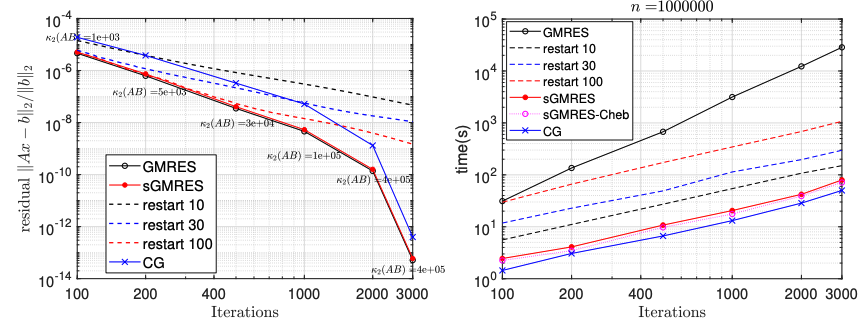
\includegraphics[width=.9\textwidth]{Graphics/GMRESvsSGMRES.png}
\end{figure}
    
\end{frame}

\begin{frame}{}
    \begin{center}
        Course recap     
    \end{center}
\end{frame}

\begin{frame}{What we have seen ...}

\only<1>{
Randomized algorithms come in various flavors
\begin{itemize}
    \bitem Random initial guess
    \bitem Application of random vectros/matrices
    \bitem Stochastic means to access quantities with high probability
\end{itemize}
}

\only<2>{
Integration
\begin{itemize}
    \bitem Riemann sums (Left, Right, Upper, Lower, Middle)
    \bitem Trapezoidal rule
    \bitem Simpson
    \bitem Variational Monte Carlo 
    \bitem \textcolor{red}{Markov Chain Monte Carlo (MCMC)}\\
    $\Rightarrow$ \textcolor{red}{Multiple techniques to speed this up!}
\end{itemize}
}

\only<3>{
Trace estimation
\begin{itemize}
    \bitem Girard-Hutchinson
    \bitem Hutch$^{++}$
    \bitem XTrace
    \bitem XNysTrace
    \bitem \textcolor{red}{Quantum Trace Estimation}
\end{itemize}
}

\only<4>{
Sketching 
\begin{itemize}
    \bitem Gaussian Embedding
    \bitem Subsampled Randomized Trigonometric Transforms (SRTT)
    \bitem Sparse Sign Embeddings (SSE)
    \begin{itemize}
        \bitem \textcolor{red}{SSE with Cauchy random variables}
        \bitem \textcolor{red}{SSE with exponential random variables}
    \end{itemize}
    \bitem \textcolor{red}{Adaptive sampling}
\end{itemize}
Application to least-squares problems
\begin{itemize}
    \bitem Sketch-and-solve
    \bitem Iterative sketching
\end{itemize}
}

\only<5>{
Guest Lecture on sketching high-dimensional probability distributions 
\begin{itemize}
    \bitem Introduction to inherent high-dimensional problems
    \bitem Introduction to tensors
    \bitem Continuous sketching
\end{itemize}
}

\only<6>{
Matrix approximation (revisited)
\begin{itemize}
    \bitem Low-rank approximation via: QR, CP-QR and ID/skeletonization
    \bitem SVD and rSVD 
    \bitem Matrix Monte Carlo
    \bitem Matrix sketching
\end{itemize}
}

\only<7>{
Multi-linear algebra
\begin{itemize}
    \bitem Detailed introduction to tensor spaces and tensor algebra
    \bitem Tensor diagrams
    \bitem Tensor product approximations
    \begin{itemize}
        \bitem Canonical Polyadic (CP) Decomposition
        \bitem Tucker Decomposition
        \bitem Tensor Train (TT) Decomposition
        \bitem  Hierarchical Tucker (HT) Decomposition
    \end{itemize}
    \bitem Generalizations of SVD
    \begin{itemize}
        \bitem (T)HOSVD
        \bitem S(T)HOSDV
        \bitem r-STHOSVD
        \bitem sketched-STHOSVD
        \bitem sub-sketch-STHOSVD
    \end{itemize}
    \bitem \textcolor{red}{Sketching TT}
\end{itemize}
}

\only<8>{
Eigenvalue problems
\begin{itemize}
    \bitem Eigenvalue revealing decompositions
    \begin{itemize}
        \bitem eigenvalue decomposition
        \bitem unitary eigenvalue decomposition
        \bitem Schur decomposition
    \end{itemize}
    \bitem Two-step numerical procedure
    \begin{itemize}
        \bitem Householder for upper Hessenbergform
        \bitem Power iteration
        \bitem Inverse iteration
        \bitem “Pure” QR algorithm (without shift)
        \bitem “Practical” QR algorithm (with shift)
    \end{itemize}
    \bitem Krylov methods for eigenvalue problems
    \begin{itemize}
        \bitem Rayleigh-Ritz (RR)/ Arnoldi method
        \bitem sketched-RR
    \end{itemize}
\end{itemize}
}

\only<9>{
Krylov methods for linear systems
\begin{itemize}
    \bitem Steepest descent
    \bitem Conjugate Gradient (CG)
    \bitem Optimality of CG
    \bitem Generalized Minimal Residual Method (GMRES)
    \begin{itemize}
        \bitem Arnoldi (Gram-Schmidt, Double Gram-Schmidt, Householder, ... )
        \bitem Lanczos
        \bitem Chebyshev recurrence
    \end{itemize}
    \bitem sketched GMRES
\end{itemize}
}

\end{frame}

\begin{frame}{Conclusion}

\begin{itemize}
    \bitem Randomized techniques are a powerful tool for certain large problems in numerical linear algebra 
    \bitem Randomized techniques are no silver bullet
    \bitem Randomized techniques often require careful implementation to be fully leveraged
\end{itemize}
    
\end{frame}

\begin{frame}{}

\begin{center}
\begin{huge}
    Thank you for your attention
\end{huge}
\end{center}
\end{frame}

\end{document}




